\documentclass[compress,11 pt,t]{beamer}
\usetheme[
	bullet=circle,		% Other option: square
	bigpagenumber,		% circled page number on lower right
	topline=true,		% colored bar at the top of the frame 
	]{Zurich}
%\useoutertheme[subsection=false]{miniframes}  
\usepackage[utf8]{inputenc} % Required for inputting international characters
\usepackage{multicol}

%-----------------------------------------------------------------------------
% BEAMER TEMPLATE
\setbeamertemplate{section in toc}[sections numbered]
\setbeamerfont{subsection in toc}{size=\small}
\usepackage{etoolbox}
\makeatletter
\patchcmd{\slideentry}{\advance\beamer@xpos by1\relax}{}{}{}
\def\beamer@subsectionentry#1#2#3#4#5{\advance\beamer@xpos by1\relax}%
\makeatother


%-----------------------------------------------------------------------------
% DOCUMENT PROPERTIES

\author[\textsc{Oriol Colomés Gené}]{\emph{author:}\\
\textsc{Oriol Colomés Gené}\\[0.2cm]
\emph{supervisor:}\\
\textsc{Santiago Badia}}
\title[Large scale FE solvers for LES of incomprssible turbulent flows]{Large scale Finite Element solvers for the large eddy simulation of incompressible turbulent flows}
\institute{Departament d'Enginyeria Civil i Ambiental}
\titlegraphic{
\includegraphics[width=0.5\textwidth]{../../sources/Figures/Cover/logo_escola_pantone_201_C}}
%\titlegraphic{
\includegraphics[width=0.7\texwidth]{../../sources/Figures/Cover/logo_escola_pantone_201_C.png}}

%-----------------------------------------------------------------------------


\begin{document}

%=========================================================================================
% TITLE
% ----------------------------------------------------------------------------
\addtocounter{framenumber}{-1}
\frame{\titlepage}
% ----------------------------------------------------------------------------
\addtocounter{framenumber}{-1}
\frame{\vfill\tableofcontents[subsectionstyle=hide,subsubsectionstyle=hide]\vfill}

%=========================================================================================
% 1.MOTIVATION
% ----------------------------------------------------------------------------
\section{Motivation}
\addtocounter{framenumber}{-1}
\frame{\vfill\tableofcontents[currentsection,
							  subsubsectionstyle=hide,
							  sectionstyle=show/shaded, 
							  subsectionstyle=show/hide]
}

%=========================================================================================
% 2.RESIDUAL-BASED VMS
% ----------------------------------------------------------------------------
\section{Residual-based VMS}
\addtocounter{framenumber}{-1}
\frame{\vfill\tableofcontents[currentsection,
							  subsubsectionstyle=hide,
							  sectionstyle=show/shaded, 
							  subsectionstyle=show/show/hide]
}

%=========================================================================================
% 2.1.FORMULATION
% ----------------------------------------------------------------------------
\subsection{Formulation}
\frame{}
\frame{}

%=========================================================================================
% 2.2.ENERGY STATEMENTS
% ----------------------------------------------------------------------------
\subsection{Energy statements}
\frame{}
\frame{}

%=========================================================================================
% 2.3.NUMERICAL EXPERIMENTS
% ----------------------------------------------------------------------------
\subsection{Numerical experiments}

%=========================================================================================
% 2.3.1.DHIT
% ----------------------------------------------------------------------------
\subsubsection{DHIT}

%=========================================================================================
% 2.3.2.TGV
% ----------------------------------------------------------------------------
\subsubsection{TGV}

%=========================================================================================
% 2.3.3.TCF
% ----------------------------------------------------------------------------
\subsubsection{TCF}

%=========================================================================================
% 2.4.CONCLUSIONS
% ----------------------------------------------------------------------------
\subsection{Conclusions}

%=========================================================================================
% 3.MIXED FE VMS
% ----------------------------------------------------------------------------
\section{Mixed FE VMS}
\addtocounter{framenumber}{-1}
\frame{\vfill\tableofcontents[currentsection,
							  subsubsectionstyle=hide,
							  sectionstyle=show/shaded, 
							  subsectionstyle=show/show/hide]
}

%=========================================================================================
% 3.1.FORMULATION
% ----------------------------------------------------------------------------
\subsection{Formulation}

%=========================================================================================
% 3.2.BLOCK-PRECONDITIONING
% ----------------------------------------------------------------------------
\subsection{Block-preconditioning}

%=========================================================================================
% 3.3.NUMERICAL EXPERIMENTS
% ----------------------------------------------------------------------------
\subsection{Numerical experiments}

%=========================================================================================
% 3.3.1.TGV
% ----------------------------------------------------------------------------
\subsubsection{TGV}

%=========================================================================================
% 3.3.2.TCF
% ----------------------------------------------------------------------------
\subsubsection{TCF}

%=========================================================================================
% 3.4.CONCLUSIONS
% ----------------------------------------------------------------------------
\subsection{Conclusions}

%=========================================================================================
% 4.SRK
% ----------------------------------------------------------------------------
\section{Segregated Runge-Kutta}
\addtocounter{framenumber}{-1}
\frame{\vfill\tableofcontents[currentsection,
							  subsubsectionstyle=hide,
							  sectionstyle=show/shaded, 
							  subsectionstyle=show/show/hide]
}

%=========================================================================================
% 4.1.FORMULATION
% ----------------------------------------------------------------------------
\subsection{Formulation}

%=========================================================================================
% 4.2.NUMERICAL EXPERIMENTS
% ----------------------------------------------------------------------------
\subsection{Numerical experiments}

%=========================================================================================
% 4.2.1.ANALYTICAL
% ----------------------------------------------------------------------------
\subsubsection{Analytical solution}

%=========================================================================================
% 4.2.2.CYLINDER
% ----------------------------------------------------------------------------
\subsubsection{Flow around a cylinder}

%=========================================================================================
% 4.3.CONCLUSIONS
% ----------------------------------------------------------------------------
\subsection{Conclusions}

%=========================================================================================
% 5.SVMS
% ----------------------------------------------------------------------------
\section{Segregated VMS}
\addtocounter{framenumber}{-1}
\frame{\vfill\tableofcontents[currentsection,
							  subsubsectionstyle=hide,
							  sectionstyle=show/shaded, 
							  subsectionstyle=show/show/hide]
}

%=========================================================================================
% 5.1.FORMULATION
% ----------------------------------------------------------------------------
\subsection{Formulation}

%=========================================================================================
% 5.2.BLOCK-PRECONDITIONING
% ----------------------------------------------------------------------------
\subsection{Block-preconditioning}

%=========================================================================================
% 5.3.NUMERICAL EXPERIMENTS
% ----------------------------------------------------------------------------
\subsection{Numerical experiments}

%=========================================================================================
% 5.3.1.TGV
% ----------------------------------------------------------------------------
\subsubsection{TGV}

%=========================================================================================
% 5.3.2.TCF
% ----------------------------------------------------------------------------
\subsubsection{TCF}

%=========================================================================================
% 5.3.3.NACA
% ----------------------------------------------------------------------------
\subsubsection{Flow around a NACA profile}

%=========================================================================================
% 5.4.CONCLUSIONS
% ----------------------------------------------------------------------------
\subsection{Conclusions}

%=========================================================================================
% 6.CONCLUSIONS
% ----------------------------------------------------------------------------
\section{Conclusions}
\addtocounter{framenumber}{-1}
\frame{\vfill\tableofcontents[currentsection,
							  subsubsectionstyle=hide,
							  sectionstyle=show/shaded, 
							  subsectionstyle=show/show/hide]
}




\begin{frame}
\frametitle{Outline}
%\framesubtitle{Handwriting}

\begin{itemize}
    \item Line 1.
    \only<2->{
    \item Line 2.\\
        {\handwriting \textcolor{tangocolordarkchameleon}{Less formal} }
    }
    \only<3->{
    \item Line 3.\\
        {\handwriting \textcolor{tangocolordarkscarletred}{
        Less formal, different color.} }
    }
\end{itemize}


\end{frame}
% ----------------------------------------------------------------------------


% ----------------------------------------------------------------------------
\begin{frame}
\frametitle{Blocks}

\begin{block}{Standard Block}
    This is a standard block.
\end{block}

\begin{exampleblock}{Example Block}
    This is an example block.
\end{exampleblock}

\begin{alertblock}{Alert Block}
    This is an alert block.
\end{alertblock}



\end{frame}
% ----------------------------------------------------------------------------


% ----------------------------------------------------------------------------
\usebackgroundtemplate{
   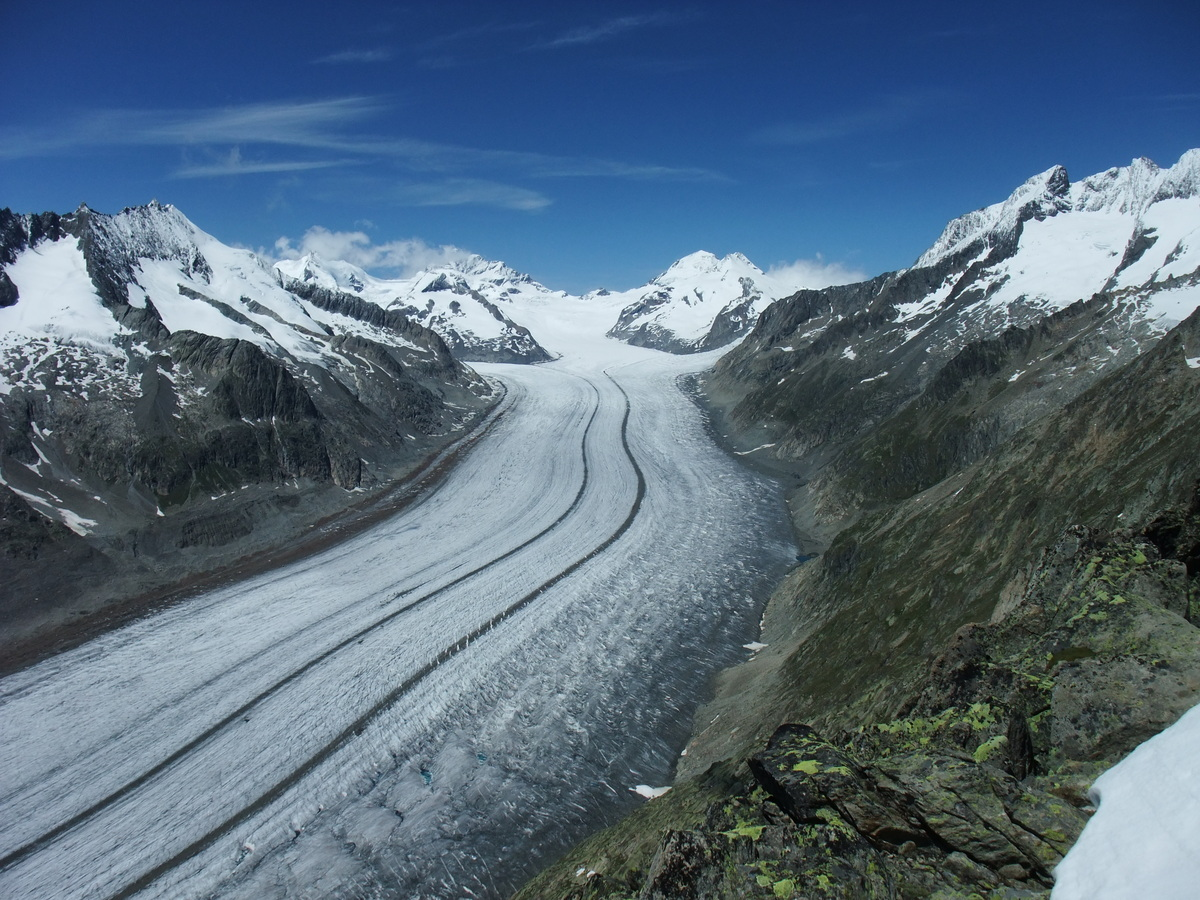
\includegraphics[width=\paperwidth,
                    height=\paperheight]{aletsch}
}
\begin{frame}
\ \\ \ \\
\centering \Large \textcolor{white}{Questions?}

\end{frame}
\usebackgroundtemplate{}
% ----------------------------------------------------------------------------


\end{document}
